
\documentclass{article}
\usepackage{amsmath, amsthm}
\usepackage{amssymb}
\usepackage{mathtools}
\usepackage[all,cmtip]{xy}
\usepackage{color}


\setcounter{tocdepth}{4}

\renewenvironment{proof}{ {\bfseries Proof:}}{\qed}

\newtheoremstyle{mytheorem}%                % Name
{}%                                     % Space above
{}%                                     % Space below
{\itshape}%                                     % Body font
{0pt}%\parindent}%                                     % Indent amount
{\bfseries}%                            % Theorem head font
{.}%                                    % Punctuation after theorem head
{ }%                                    % Space after theorem head, ' ', or \newline
{}%                                     % Theorem head spec (can be left empty, meaning `normal')

\theoremstyle{mytheorem}
\newtheorem{thm}{Theorem}[section]
\newtheorem{proposition}[thm]{Proposition}
\newtheorem{lemma}[thm]{Lemma}
\newtheorem{corollary}[thm]{Corollary}


\newtheoremstyle{mydefinition}%                % Name
{}%                                     % Space above
{}%                                     % Space below
{}%                                     % Body font
{0pt}%\parindent}%                                     % Indent amount
{\bfseries}%                            % Theorem head font
{.}%                                    % Punctuation after theorem head
{ }%                                    % Space after theorem head, ' ', or \newline
{}%                                     % Theorem head spec (can be left empty, meaning `normal')

\theoremstyle{mydefinition}
\newtheorem{definition}[thm]{Definition}
\newtheorem{example}[thm]{Example}
\newtheorem{exercise}[thm]{Exercise}
\newtheorem{remark}[thm]{Remark}
%\newtheorem{ques}[thm]{Q.}
\newtheorem*{ques}{Question}
%\newtheorem{ans}[thm]{Ans.}
\newtheorem*{ans}{Ans}



\numberwithin{equation}{section}

%Real numbers, complex numbers, etc.
\newcommand{\R}{\mathbb{R}}
\newcommand{\C}{\mathbb{C}}
\newcommand{\Z}{\mathbb{Z}}
\newcommand{\Q}{\mathbb{Q}}
\renewcommand{\P}{\mathbb{P}}

%How does latex not have these?
\DeclareMathOperator{\Ad}{Ad}
\DeclareMathOperator{\ad}{ad}
\DeclareMathOperator{\tr}{tr}
\DeclareMathOperator{\Tr}{Tr}
\DeclareMathOperator{\Hom}{Hom}
\DeclareMathOperator{\Spec}{Spec}
\DeclareMathOperator{\im}{im}
\DeclareMathOperator{\rank}{rank}
\DeclareMathOperator{\Exists}{\exists}
\DeclareMathOperator{\Forall}{\forall}

\DeclareMathOperator*{\colim}{colim}
\DeclareMathOperator*{\holim}{holim}
\DeclareMathOperator*{\hocolim}{hocolim}


%fractions and inner product
\newcommand{\pr}[2][\:]{\frac{\partial #1}{\partial #2}}
\newcommand{\innerp}[2]{\langle #1, #2 \rangle}

\newcommand*\conj[1]{\overline{#1}}
\newcommand*\norm[1]{\lVert #1 \rVert}

\renewcommand{\figurename}{Fig.}
\usepackage{float}
\usepackage{wrapfig}

\usepackage{enumitem}
\setlist[enumerate]{itemsep=0mm}
\usepackage{geometry}
\geometry{
	a4paper,
	total={170mm,257mm},
	left=20mm,
	top=20mm
}


\usepackage{fancyhdr}
\pagestyle{fancy}
\lhead{\scshape Apurva Nakade}
%\rhead{\scshape Mathcamp 2017}
\renewcommand*{\thepage}{\small\arabic{page}}

\usepackage{wrapfig}
\usepackage{caption}
\usepackage{csquotes}
\usepackage{mdframed}

\renewcommand{\thefootnote}{\fnsymbol{footnote}}

\begin{document}
\title{Euler Characteristic for surfaces}
\author{Apurva Nakade}
\maketitle






\begin{wrapfigure}[10]{r}{0.20\textwidth}
	\begin{center}
		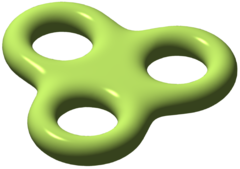
\includegraphics[width=0.20\textwidth]{images/3_holed_torus}
	\end{center}
	\captionsetup{labelformat=empty}
	\caption{Example of a surface: \\3 holed torus}
\end{wrapfigure}
Our goal is to determine the Euler characteristic for more complicated surfaces than a sphere. The most general surface that we'll consider is the $g$ holed torus. The Euler characteristic can be defined for much more complicated objects and similar results hold true.

As with the sphere a \textbf{surface graph} on a surface is a \emph{connected planar} graph $ G = (V,E) $ such that $ V $ and $ E $ are now on the surface and all the faces are \textbf{polygons}.

\begin{exercise}\label{JordanCurve}
	Being polygonal is a non-trivial condition for a graph on a surface which is not a sphere. Find a planar connected graph with at least 1 face on a torus with 3 vertices which is not polygonal. Does such a graph exist on a sphere?
\end{exercise}
% This problem does not arise for a sphere because of the \textbf{Jordan Curve Theorem}. Try to read a proof of the Jordan curve theorem and see where the proof goes wrong for general surfaces.


\section{Euler's theorem for surfaces}

Let $G$ be a surface graph on the surface $S$ and define $\chi(S)$ to be the Euler characteristic of $G$.
\begin{mdframed}
	\begin{thm}[Euler characteristic]
		\label{thm:Euler}
		The Euler characteristic of a $g$ holed torus is $2 - 2g$.\\
	\end{thm}
\end{mdframed}
The idea behind the proof of this theorem is very similar to what we did for a sphere. However, to prove that the Euler characteristic does not depend on the graph we cannot delete vertices and edges successively as we cannot guarantee that a surface graph would have polygonal faces after deleting edges. Instead we'll \textit{add} edges and vertices. We break up the proof into two steps.


\begin{lem}\label{thm:Euler_thm_surface}
	For any two surface graphs $G,G'$ on a surface $S$ we have $\chi(G)=\chi(G')$. Hence we can define $\chi(S):=\chi(G)$ for any surface graph $G$.
\end{lem}

\begin{exercise}[proof of Lemma \ref{thm:Euler_thm_surface}]\label{thm:proof_euler_char_1}
	Let $ S $ be any surface.
	\begin{enumerate}
		\item Give an example of a surface graph which does not have polygonal faces upon deleting an edge.
		\item Show that a surface graphs stays a surface graph and it's Euler characteristic does not change by performing one of the following operations
		      \begin{enumerate}[label=\alph*)]
		      	\item adding a new edge joining two existing vertices
		      	\item subdividing an edge by declaring it's midpoint as a new vertex
		      \end{enumerate}
		\item Argue that given two different surface graphs $ G $ and $ G' $ of  $ S $ it is possible to find a  \emph{common refinement} $ G'' $ of the two using a sequence of the above two steps.
		\item Conclude that $ \chi(G) = \chi(G'') = \chi(G') $.
	\end{enumerate}
\end{exercise}

We can now use \emph{any} surface graph to \textbf{define} the Euler characteristic of the surface.

\begin{exercise} [proof of Theorem \ref{thm:Euler}]
	$\quad$
	\begin{enumerate}
		\item Draw a surface graph on a torus and show that it's Euler characteristic is 0.
		\item Glue $g$ many of these surface graphs appropriately to get a surface graph on a $g$ holed torus.
		\item Prove that the Euler characteristic of this surface graph is $2-2g$.
	\end{enumerate}
\end{exercise}


\begin{exercise}[suggested by Jan]
	Show that for any graph $G$ on a surface $S$, not necessarily with polygonal faces, we have $\chi(G) \ge \chi(S)$. So an alternate way of defining the Euler characteristic is by defining it to be the \emph{minimum} Euler characteristic of any graph on the surface.
\end{exercise}

\subsection{Platonic Solids}
A platonic solid is a convex polyhedron all of whose faces are regular polygons which are congruent to each other, i.e. all the edges have the same length and all the faces have the same number of sides e.g. a tetrahedron, a cube, etc. We'll assume that the word convex means that the platonic solid is topologically equivalent to $S^2$. We can use the Euler characteristic to prove that there at most 5 such solids.

Consider a platonic solid $ S $ and let $V,E,F$ be it's vertices, edges and faces. Suppose all the faces of $ S $ are polygons with $ {n} $ number of edges. Further suppose that $ {p} $ edges of $S $ intersect at a single vertex.

\begin{exercise}
	Argue that both $ n $ and $ p $ should be at least 3.
\end{exercise}

\begin{exercise}
	\begin{enumerate}
		\item By counting the total number of edges, show that $ p |V| = 2 |E| $ and $ n |F| = 2|E| $.
		\item Use $\chi(S^2) = 2$ to show that
		      \begin{align}\label{eq:platonic_solid}
		      	\dfrac{1}{n} - \dfrac{1}{2} + \dfrac{1}{p} = \dfrac{1}{|E|}
		      \end{align}
		      and because $ |E| > 0 $ this implies $ \frac{1}{n} + \frac{1}{p} >  \frac{1}{2}$.
		\item Show that there at most 5 possible triples $ (n, p, |E|)$ that satisfy (\ref{eq:platonic_solid}). As it turns out all the 5 triples are realizable as regular polyhedra.
	\end{enumerate}
	You can also do this exercise more geometrically using angle defects.
\end{exercise}

\begin{exercise}
	Does the polyhedron in Fig.\ref{rubik} have i) more `holes' than you think it should have ii) less `holes' than you think it should have or iii) the same number of `holes' as what you think it should have? Verify your answer using the Euler characteristic.
\end{exercise}
\begin{figure}[H]
	\centering
	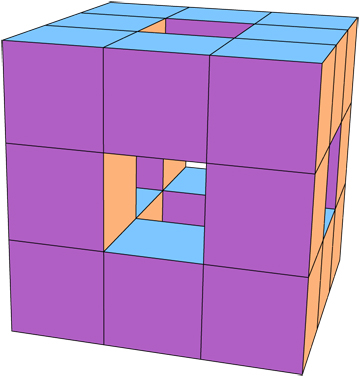
\includegraphics[width=0.15\linewidth]{images/cube_with_holes}
	\caption{Rubik's cube with `holes'}
	\label{rubik}
\end{figure}

\begin{exercise}
	If you know what a Klein bottle and the real projective plane is, find their Euler characteristics.
\end{exercise}

\section{Angle defects}

\begin{exercise}
	\begin{enumerate}
		\item For the cubical torus in Fig.\ref{cubical_torus} find the vertices which have +ve, 0, and -ve curvature without making any computations.
		\item Verify your answers by computing the angle defects.
		\item Compute the total angle defect and verify Descartes' theorem.
	\end{enumerate}
	\begin{figure}[H]
		\centering
		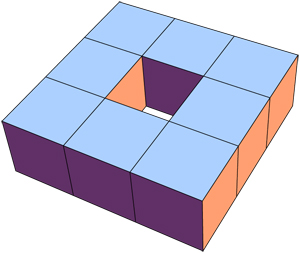
\includegraphics[width=0.25\linewidth]{images/torus_cube}
		\caption{Cubical torus}
		\label{cubical_torus}
	\end{figure}
\end{exercise}

\begin{exercise}
	For a general polyhedron try to describe what vertices with 0 angle defect can possibly look like.
\end{exercise}

\end{document}
